%%%%%%%%%%%%%%%%%%%%%%%%%%%%%%%%%%%%%%
%%%%%%%%%%%%%%%%%%%%%%%%%%%%%%%%%%%%%%
% Do not edit the TeX file your work
% will be overwritten.  Edit the RnW
% file instead.
%%%%%%%%%%%%%%%%%%%%%%%%%%%%%%%%%%%%%%
%%%%%%%%%%%%%%%%%%%%%%%%%%%%%%%%%%%%%%




We now consider functional perturbations to the prior on the sticks. Figure~\ref{fig:functional_sens_plot_thresh0} shows the effect of our choice of $\phi$ on the expected number of distinct clusters. 



\begin{knitrout}
\definecolor{shadecolor}{rgb}{0.969, 0.969, 0.969}\color{fgcolor}\begin{figure}[!h]

{\centering 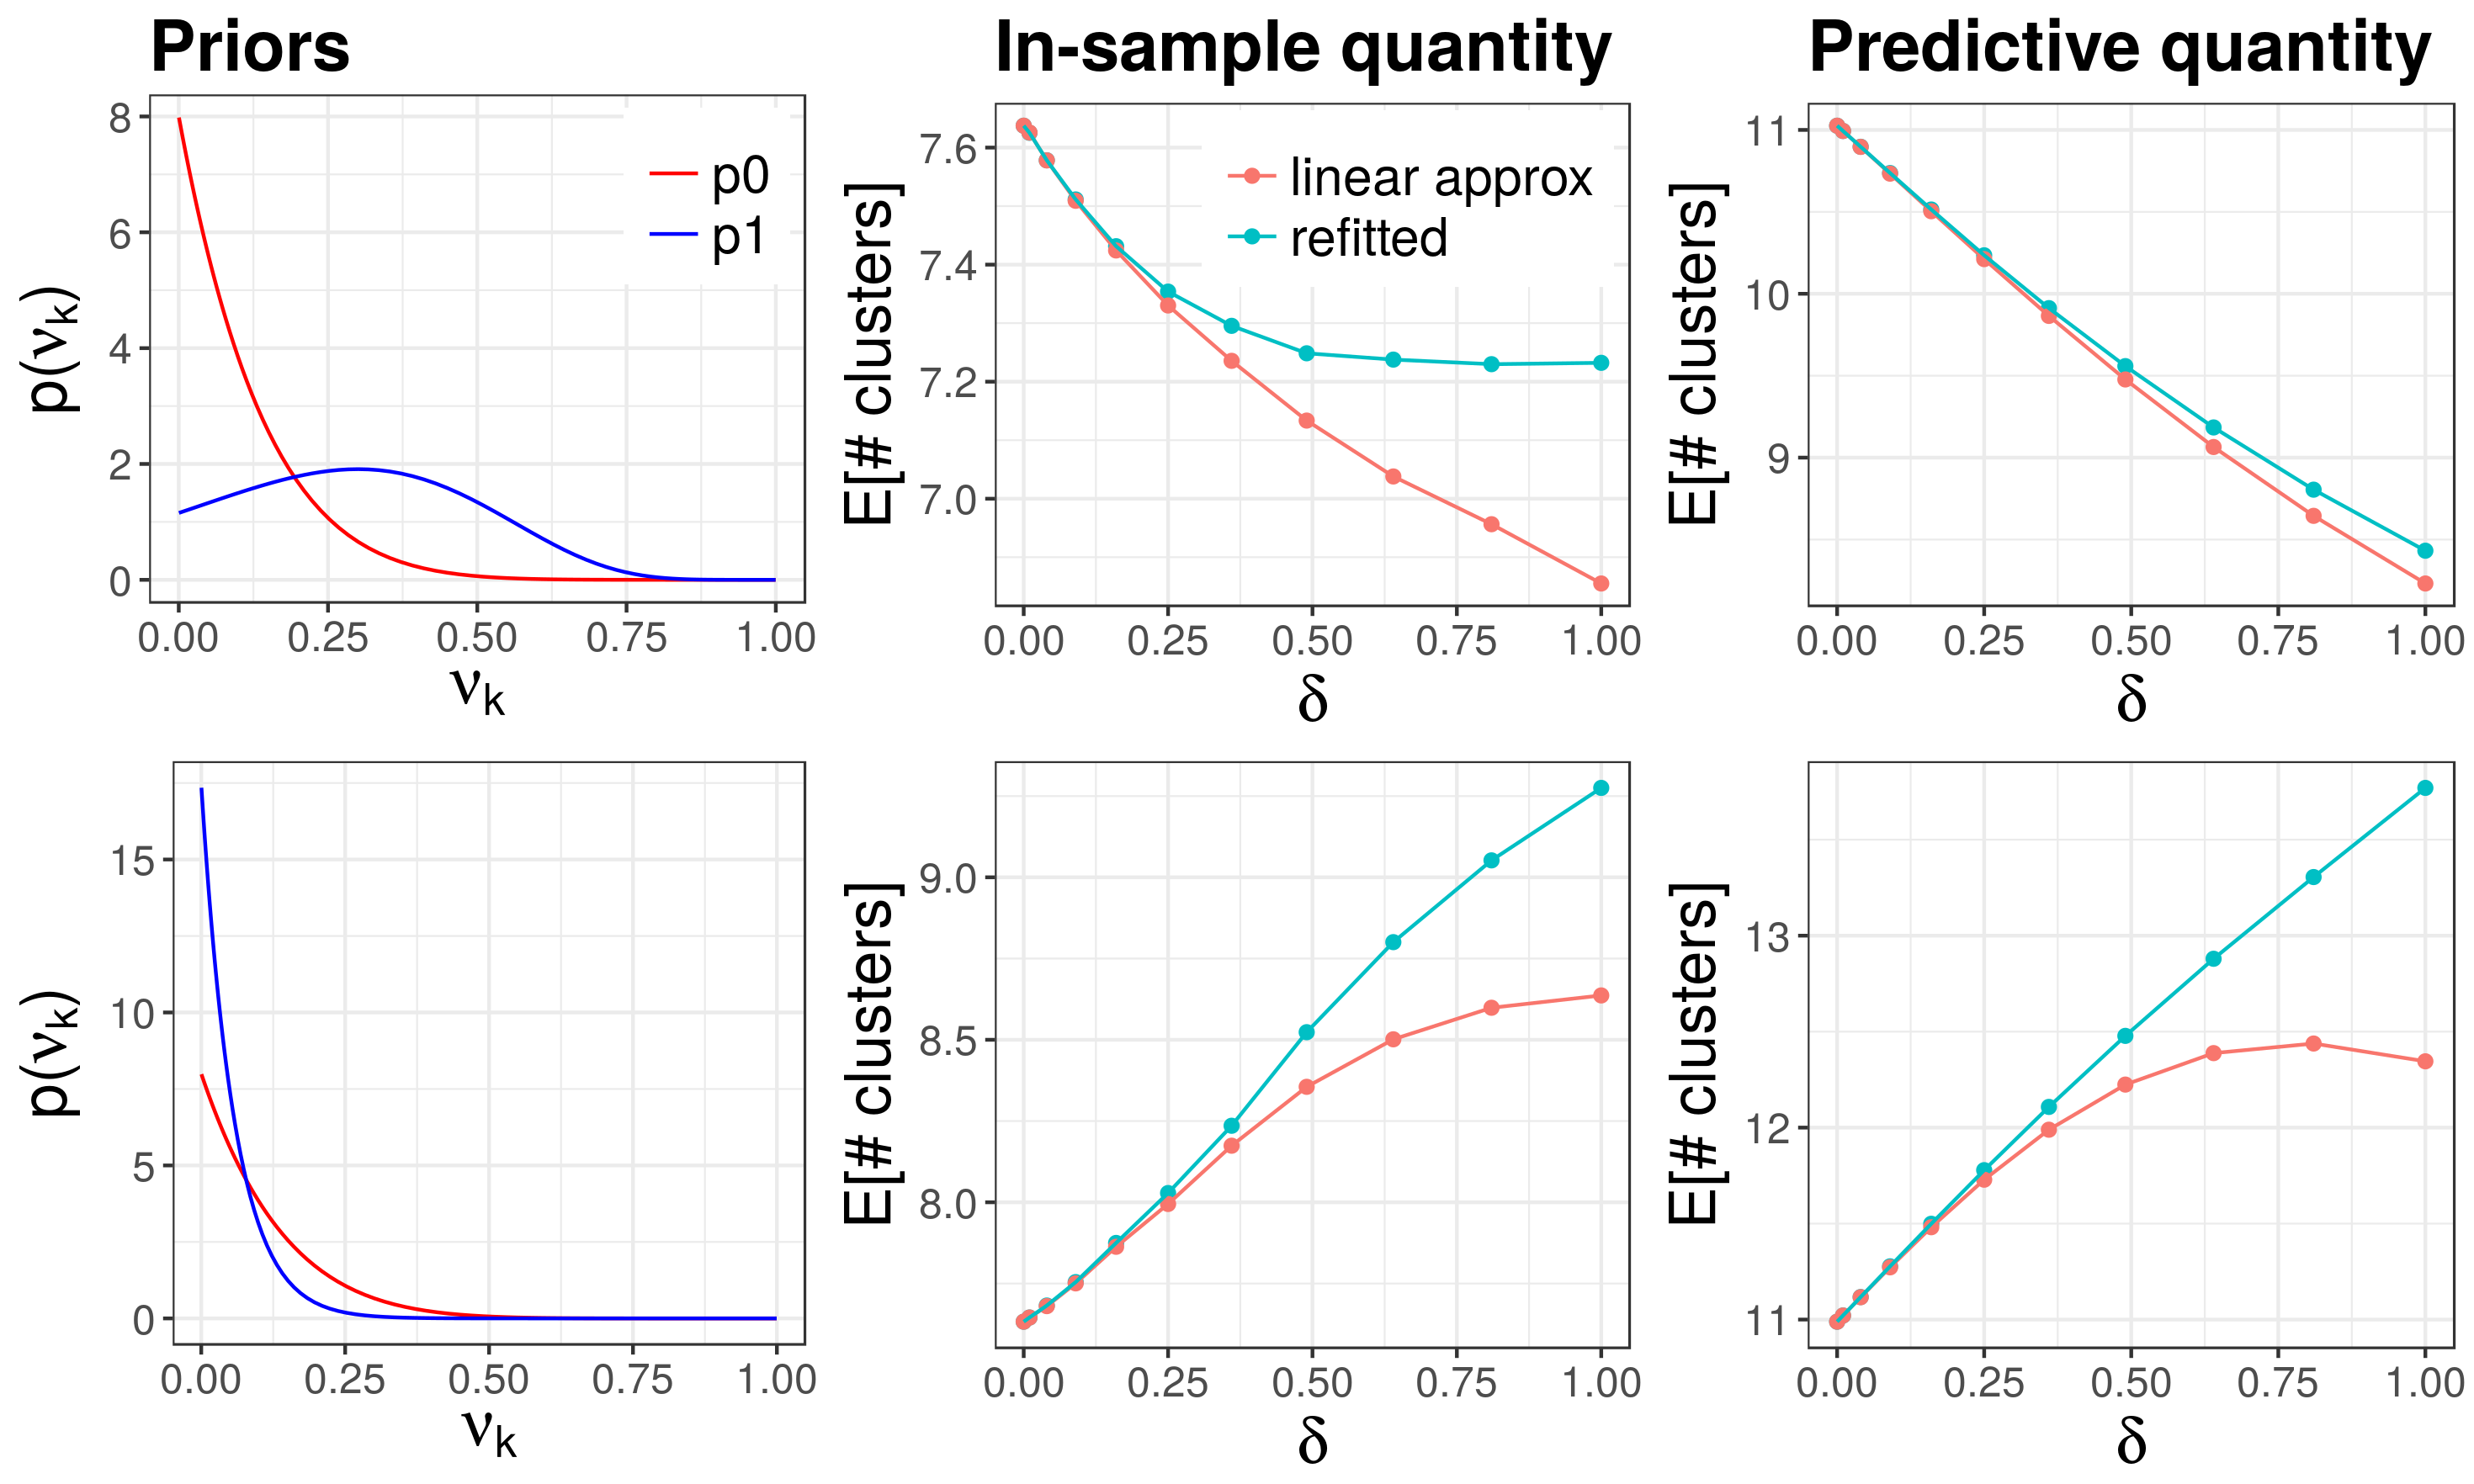
\includegraphics[width=0.98\linewidth,height=0.588\linewidth]{figure/functional_sens_plot_thresh0-1} 

}

\caption{\label{fig:func_sens_e_num_clusters_thresh0}
The effect of prior perturbation on the expected number of distinct clusters ($t = 0$). 
Left column: the original prior $p_{0}$ in red,
the perturbed prior $p^c$ in blue. 
Middle: linearly approximated vs.
re-fitted in-sample expected number of clusters. 
Right: linearly approximated vs.
re-fitted predictive expected number of clusters.  }\label{fig:functional_sens_plot_thresh0}
\end{figure}


\end{knitrout}
%



\begin{knitrout}
\definecolor{shadecolor}{rgb}{0.969, 0.969, 0.969}\color{fgcolor}\begin{figure}[!h]

{\centering \includegraphics[width=0.98\linewidth,height=0.588\linewidth]{figure/functional_sens_plot_thresh3-1} 

}

\caption{\label{fig:func_sens_e_num_clusters_thresh3}
The effect of prior perturbation on the expected number of clusters with at least three 
data points. ($t = 3$). 
Left column: the original prior $p_{0}$ in red,
the perturbed prior $p^c$ in blue. 
Middle: linearly approximated vs.
re-fitted in-sample expected number of clusters. 
Right: linearly approximated vs.
re-fitted predictive expected number of clusters.  }\label{fig:functional_sens_plot_thresh3}
\end{figure}


\end{knitrout}
